\documentclass[tikz,border=3mm]{standalone}

\usepackage{amsmath,amssymb}
\usepackage{xcolor}
\usepackage{helvet}
\renewcommand{\familydefault}{\sfdefault}
\usetikzlibrary{arrows.meta,positioning,fit,calc}

\definecolor{ink}{HTML}{111827}
\definecolor{muted}{HTML}{4B5563}
\definecolor{hwbg}{HTML}{F8FAFC}
\definecolor{rosbg}{HTML}{DFF1FB}
\definecolor{ctrlbg}{HTML}{F1E4FA}
\definecolor{netbg}{HTML}{E7F5EA}
\definecolor{outbg}{HTML}{FFF7E6}
\definecolor{blue}{HTML}{0EA5E9}
\definecolor{green}{HTML}{16A34A}
\definecolor{red}{HTML}{DC2626}
\definecolor{violet}{HTML}{7C3AED}
\definecolor{amber}{HTML}{D97706}
\definecolor{dark}{HTML}{374151}

\tikzset{
  >=Latex,
  title/.style={font=\bfseries\large, align=center, text=black},
  block/.style={
    rectangle, draw=black, fill=white, line width=0.58pt,
    minimum height=1.02cm, text width=4.15cm,
    align=center, rounded corners=1pt, inner sep=3pt,
    font=\small, text=ink
  },
  smallblock/.style={
    rectangle, draw=black, fill=white, line width=0.55pt,
    minimum height=0.92cm, text width=3.05cm,
    align=center, rounded corners=1pt, inner sep=2.4pt,
    font=\small, text=ink
  },
  tinyblock/.style={
    rectangle, draw=black, fill=white, line width=0.55pt,
    minimum height=1.08cm, text width=2.34cm,
    align=center, rounded corners=1pt, inner sep=2.2pt,
    font=\scriptsize, text=ink
  },
  wideblock/.style={
    rectangle, draw=black, fill=white, line width=0.58pt,
    minimum height=1.04cm, text width=5.20cm,
    align=center, rounded corners=1pt, inner sep=3pt,
    font=\small, text=ink
  },
  note/.style={
    rectangle, draw=black!40, fill=white, line width=0.45pt,
    text width=4.8cm, align=left, rounded corners=1pt,
    inner sep=3pt, font=\scriptsize, text=muted
  },
  formula/.style={font=\scriptsize, text=muted},
  arrow/.style={->, line width=0.68pt, draw=black, shorten >=2pt, shorten <=2pt},
  bus/.style={->, line width=0.9pt, draw=blue, shorten >=2pt, shorten <=2pt},
  feedback/.style={->, line width=0.8pt, draw=red, shorten >=2pt, shorten <=2pt},
  dashedframe/.style={draw=black, dashed, line width=0.9pt, rounded corners=2pt}
}

\begin{document}
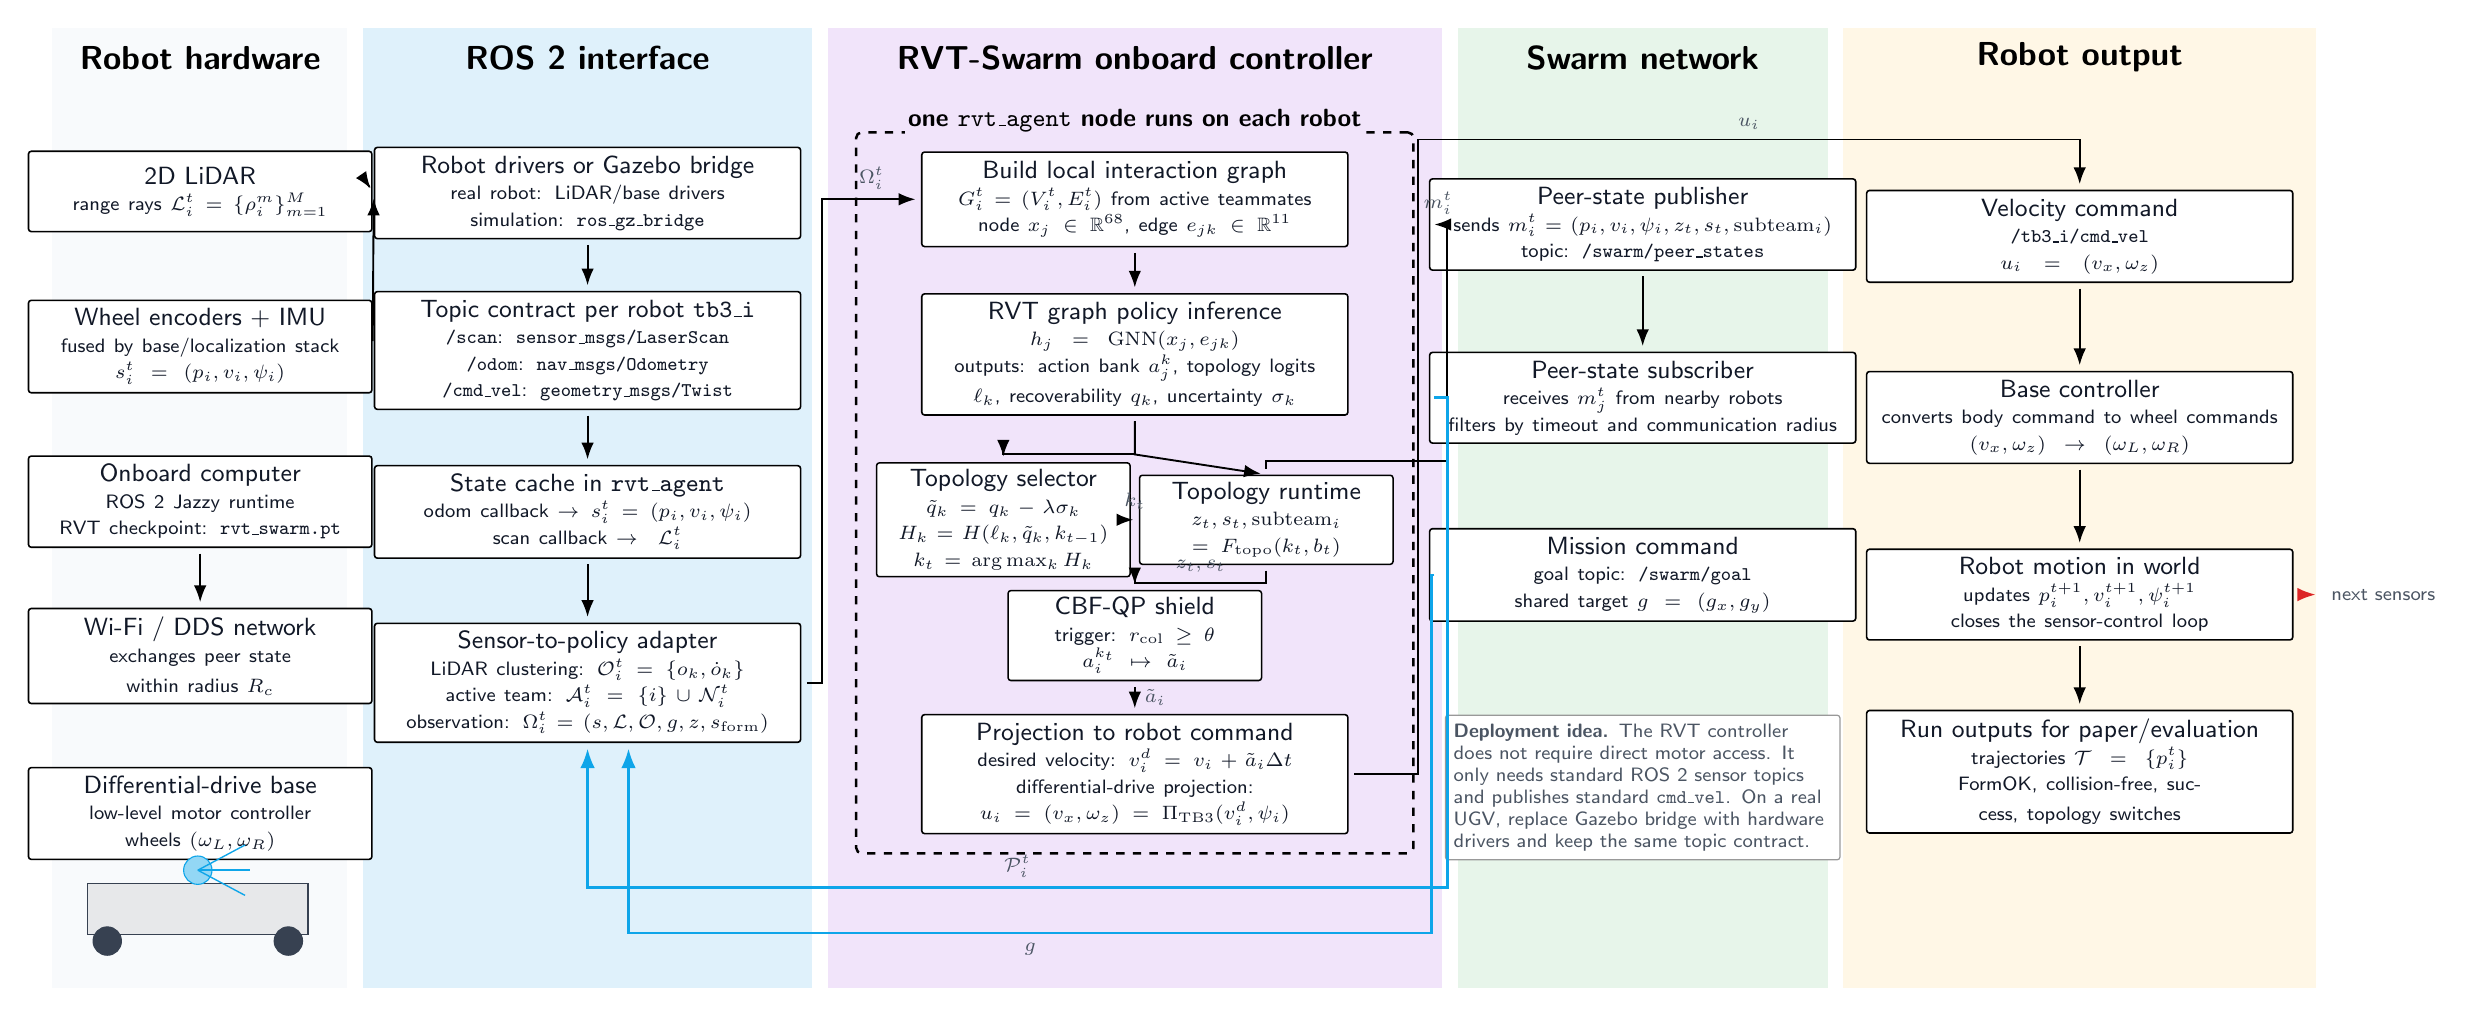
\begin{tikzpicture}[x=1cm,y=1cm]
  \def\Ytop{12.2}
  \def\Ybot{0.0}

  \fill[hwbg]   (0.0,\Ybot) rectangle (3.75,\Ytop);
  \fill[rosbg]  (3.95,\Ybot) rectangle (9.65,\Ytop);
  \fill[ctrlbg] (9.85,\Ybot) rectangle (17.65,\Ytop);
  \fill[netbg]  (17.85,\Ybot) rectangle (22.55,\Ytop);
  \fill[outbg]  (22.75,\Ybot) rectangle (28.75,\Ytop);

  \node[title] at (1.88,11.82) {Robot hardware};
  \node[title] at (6.80,11.82) {ROS 2 interface};
  \node[title] at (13.75,11.82) {RVT-Swarm onboard controller};
  \node[title] at (20.20,11.82) {Swarm network};
  \node[title] at (25.75,11.82) {Robot output};

  % Hardware column.
  \node[block] (lidarhw) at (1.88,10.12)
    {2D LiDAR\\[-0.5mm]
    {\scriptsize range rays $\mathcal L_i^t=\{\rho_i^m\}_{m=1}^{M}$}};
  \node[block] (odomhw) at (1.88,8.15)
    {Wheel encoders + IMU\\[-0.5mm]
    {\scriptsize fused by base/localization stack}\\[-0.5mm]
    {\scriptsize $s_i^t=(p_i,v_i,\psi_i)$}};
  \node[block] (cpu) at (1.88,6.18)
    {Onboard computer\\[-0.5mm]
    {\scriptsize ROS 2 Jazzy runtime}\\[-0.5mm]
    {\scriptsize RVT checkpoint: \texttt{rvt\_swarm.pt}}};
  \node[block] (radiohw) at (1.88,4.22)
    {Wi-Fi / DDS network\\[-0.5mm]
    {\scriptsize exchanges peer state within radius $R_c$}};
  \node[block] (basehw) at (1.88,2.22)
    {Differential-drive base\\[-0.5mm]
    {\scriptsize low-level motor controller}\\[-0.5mm]
    {\scriptsize wheels $(\omega_L,\omega_R)$}};

  % Simple robot silhouette.
  \begin{scope}[shift={(0.45,0.68)}]
    \draw[fill=dark!12,draw=dark,line width=0.5pt] (0,0) rectangle (2.80,0.65);
    \draw[fill=dark,draw=dark] (0.25,-0.08) circle (0.18);
    \draw[fill=dark,draw=dark] (2.55,-0.08) circle (0.18);
    \draw[fill=blue!45,draw=blue] (1.40,0.82) circle (0.18);
    \draw[blue,line width=0.5pt] (1.40,0.82) -- ++(0.60,0.32);
    \draw[blue,line width=0.5pt] (1.40,0.82) -- ++(0.66,0.00);
    \draw[blue,line width=0.5pt] (1.40,0.82) -- ++(0.60,-0.32);
  \end{scope}

  % ROS interface column.
  \node[wideblock] (driver) at (6.80,10.10)
    {Robot drivers or Gazebo bridge\\[-0.5mm]
    {\scriptsize real robot: LiDAR/base drivers}\\[-0.5mm]
    {\scriptsize simulation: \texttt{ros\_gz\_bridge}}};
  \node[wideblock] (topics) at (6.80,8.10)
    {Topic contract per robot \texttt{tb3\_i}\\[-0.5mm]
    {\scriptsize \texttt{/scan}: \texttt{sensor\_msgs/LaserScan}}\\[-0.5mm]
    {\scriptsize \texttt{/odom}: \texttt{nav\_msgs/Odometry}}\\[-0.5mm]
    {\scriptsize \texttt{/cmd\_vel}: \texttt{geometry\_msgs/Twist}}};
  \node[wideblock] (cache) at (6.80,6.05)
    {State cache in \texttt{rvt\_agent}\\[-0.5mm]
    {\scriptsize odom callback $\rightarrow s_i^t=(p_i,v_i,\psi_i)$}\\[-0.5mm]
    {\scriptsize scan callback $\rightarrow \mathcal L_i^t$}};
  \node[wideblock] (obsproc) at (6.80,3.88)
    {Sensor-to-policy adapter\\[-0.5mm]
    {\scriptsize LiDAR clustering: $\mathcal O_i^t=\{o_k,\dot o_k\}$}\\[-0.5mm]
    {\scriptsize active team: $\mathcal A_i^t=\{i\}\cup\mathcal N_i^t$}\\[-0.5mm]
    {\scriptsize observation: $\Omega_i^t=(s,\mathcal L,\mathcal O,g,z,s_{\mathrm{form}})$}};

  % Controller column.
  \node[wideblock,minimum height=1.20cm] (graph) at (13.75,10.02)
    {Build local interaction graph\\[-0.5mm]
    {\scriptsize $G_i^t=(V_i^t,E_i^t)$ from active teammates}\\[-0.5mm]
    {\scriptsize node $x_j\in\mathbb R^{68}$, edge $e_{jk}\in\mathbb R^{11}$}};
  \node[wideblock,minimum height=1.42cm] (policy) at (13.75,8.05)
    {RVT graph policy inference\\[-0.5mm]
    {\scriptsize $h_j=\mathrm{GNN}(x_j,e_{jk})$}\\[-0.5mm]
    {\scriptsize outputs: action bank $a_j^k$, topology logits $\ell_k$, recoverability $q_k$, uncertainty $\sigma_k$}};
  \node[smallblock] (select) at (12.08,5.95)
    {Topology selector\\[-0.5mm]
    {\scriptsize $\tilde q_k=q_k-\lambda\sigma_k$}\\[-0.5mm]
    {\scriptsize $H_k=H(\ell_k,\tilde q_k,k_{t-1})$}\\[-0.5mm]
    {\scriptsize $k_t=\arg\max_k H_k$}};
  \node[smallblock] (runtime) at (15.42,5.95)
    {Topology runtime\\[-0.5mm]
    {\scriptsize $z_t,s_t,\mathrm{subteam}_i$}\\[-0.5mm]
    {\scriptsize $=F_{\mathrm{topo}}(k_t,b_t)$}};
  \node[smallblock] (shield) at (13.75,4.48)
    {CBF-QP shield\\[-0.5mm]
    {\scriptsize trigger: $r_{\mathrm{col}}\ge\theta$}\\[-0.5mm]
    {\scriptsize $a_i^{k_t}\mapsto\tilde a_i$}};
  \node[wideblock] (twist) at (13.75,2.72)
    {Projection to robot command\\[-0.5mm]
    {\scriptsize desired velocity: $v_i^d=v_i+\tilde a_i\Delta t$}\\[-0.5mm]
    {\scriptsize differential-drive projection:}\\[-0.5mm]
    {\scriptsize $u_i=(v_x,\omega_z)=\Pi_{\mathrm{TB3}}(v_i^d,\psi_i)$}};
  \node[dashedframe, fit=(graph)(policy)(select)(runtime)(shield)(twist),
        inner xsep=0.25cm, inner ysep=0.24cm] {};
  \node[font=\bfseries\small,fill=ctrlbg,inner sep=1pt] at (13.75,11.02)
    {one \texttt{rvt\_agent} node runs on each robot};

  % Network column.
  \node[wideblock] (peerpub) at (20.20,9.70)
    {Peer-state publisher\\[-0.5mm]
    {\scriptsize sends $m_i^t=(p_i,v_i,\psi_i,z_t,s_t,\mathrm{subteam}_i)$}\\[-0.5mm]
    {\scriptsize topic: \texttt{/swarm/peer\_states}}};
  \node[wideblock] (peersub) at (20.20,7.50)
    {Peer-state subscriber\\[-0.5mm]
    {\scriptsize receives $m_j^t$ from nearby robots}\\[-0.5mm]
    {\scriptsize filters by timeout and communication radius}};
  \node[wideblock] (goalnet) at (20.20,5.25)
    {Mission command\\[-0.5mm]
    {\scriptsize goal topic: \texttt{/swarm/goal}}\\[-0.5mm]
    {\scriptsize shared target $g=(g_x,g_y)$}};
  \node[note] (deploynote) at (20.20,2.55)
    {\textbf{Deployment idea.} The RVT controller does not require direct motor access. It only needs standard ROS 2 sensor topics and publishes standard \texttt{cmd\_vel}. On a real UGV, replace Gazebo bridge with hardware drivers and keep the same topic contract.};

  % Output column.
  \node[wideblock] (cmdout) at (25.75,9.55)
    {Velocity command\\[-0.5mm]
    {\scriptsize \texttt{/tb3\_i/cmd\_vel}}\\[-0.5mm]
    {\scriptsize $u_i=(v_x,\omega_z)$}};
  \node[wideblock] (basectrl) at (25.75,7.25)
    {Base controller\\[-0.5mm]
    {\scriptsize converts body command to wheel commands}\\[-0.5mm]
    {\scriptsize $(v_x,\omega_z)\rightarrow(\omega_L,\omega_R)$}};
  \node[wideblock] (motion) at (25.75,5.00)
    {Robot motion in world\\[-0.5mm]
    {\scriptsize updates $p_i^{t+1},v_i^{t+1},\psi_i^{t+1}$}\\[-0.5mm]
    {\scriptsize closes the sensor-control loop}};
  \node[wideblock] (logs) at (25.75,2.75)
    {Run outputs for paper/evaluation\\[-0.5mm]
    {\scriptsize trajectories $\mathcal T=\{p_i^t\}$}\\[-0.5mm]
    {\scriptsize FormOK, collision-free, success, topology switches}};

  % Main data arrows.
  \draw[arrow] (lidarhw.east) -- (driver.west);
  \draw[arrow] (odomhw.east) -- (driver.west);
  \draw[arrow] (driver) -- (topics);
  \draw[arrow] (topics) -- (cache);
  \draw[arrow] (cache) -- (obsproc);
  \coordinate (obsbus) at (9.78,3.88);
  \draw[arrow] (obsproc.east) -- (obsbus) -- (9.78,10.02)
    -- node[formula,above] {$\Omega_i^t$} (graph.west);
  \draw[arrow] (graph) -- (policy);
  \coordinate (policybus) at (13.75,6.78);
  \draw[arrow] (policy.south) -- (policybus) -| (select.north);
  \draw[arrow] (policy.south) -- (policybus) -- (runtime.north);
  \draw[arrow] (select) -- node[formula,above] {$k_t$} (runtime);
  \coordinate (rtout) at (15.42,5.15);
  \coordinate (shieldin) at (13.75,5.15);
  \draw[arrow] (runtime.south) -- (rtout)
    -- node[formula,above] {$z_t,s_t$} (shieldin) -- (shield.north);
  \draw[arrow] (shield.south) -- node[formula,right] {$\tilde a_i$}
    ($(shield.south |- twist.north)$);
  \coordinate (cmdrouteA) at (17.35,2.72);
  \coordinate (cmdrouteB) at (17.35,10.78);
  \coordinate (cmdrouteC) at (25.75,10.78);
  \draw[arrow] (twist.east) -- (cmdrouteA) -- (cmdrouteB)
    -- node[formula,above] {$u_i$} (cmdrouteC) -- (cmdout.north);
  \draw[arrow] (cmdout) -- (basectrl);
  \draw[arrow] (basectrl) -- (motion);
  \draw[arrow] (motion) -- (logs);

  % Network arrows.
  \draw[arrow] (cpu.south) -- (radiohw.north);
  \coordinate (pubrouteA) at (15.42,6.70);
  \coordinate (pubrouteB) at (17.72,6.70);
  \coordinate (pubrouteC) at (17.72,9.70);
  \draw[arrow] (runtime.north) -- (pubrouteA) -- (pubrouteB) -- (pubrouteC)
    -- node[formula,above] {$m_i^t$} (peerpub.west);
  \draw[arrow] (peerpub) -- (peersub);
  \coordinate (peerlaneA) at (17.72,1.28);
  \coordinate (peerlaneB) at (6.80,1.28);
  \draw[bus] (peersub.west) -- (17.72,7.50) -- (peerlaneA)
    -- node[formula,above] {$\mathcal P_i^t$} (peerlaneB) -- (obsproc.south);
  \coordinate (goallaneA) at (17.52,0.70);
  \coordinate (goallaneB) at (7.32,0.70);
  \draw[bus] (goalnet.west) -- (17.52,5.25) -- (goallaneA)
    -- node[formula,below] {$g$} (goallaneB) -- ($(obsproc.south)+(0.52,0)$);

  % Physical feedback is implicit through the next /odom and /scan messages.
  \draw[feedback] (motion.east) -- ++(0.35,0)
    node[formula,right] {next sensors};
\end{tikzpicture}
\end{document}
